% chktex-file 1
% !TeX spellcheck = en_GB
% !TeX program = pdflatex
%
% LuxSleek-CV 1.1 LaTeX template
% Author: Andreï V. Kostyrka, University of Luxembourg
%
% 1.1: added tracking and letter-spacing for prettier lower caps, added `~` for language levels
% 1.0: initial release
%
% This template fills the gap in the available variety of templates
% by proposing something that is not a custom class, not using any
% hard-coded settings deeply hidden in style files, and provides
% a handful of custom command definitions that are as transparent as it gets.
% Developed at the University of Luxembourg.
%
% *NOTHING IS HARCODED, and never should be.*
%
% Target audience: applicants in the IT industry, or business in general
%
% The main strength of this template is, it explicitly showcases how
% to break the flow of text to achieve the most flexible right alignment
% of dates for multiple configurations.

\documentclass[11pt, a4paper]{article}

\usepackage[T1]{fontenc}     % We are using pdfLaTeX,
\usepackage[utf8]{inputenc}  % hence this preparation
\usepackage[british]{babel}
\usepackage[left = 0mm, right = 0mm, top = 0mm, bottom = 0mm]{geometry}
\usepackage[stretch = 25, shrink = 25, tracking=true, letterspace=30]{microtype}
\usepackage{graphicx}        % To insert pictures
\usepackage{xcolor}          % To add colour to the document
\usepackage{marvosym}        % Provides icons for the contact details
\usepackage{fontawesome}

\usepackage{enumitem}        % To redefine spacing in lists
\setlist{parsep = 0pt, topsep = 0pt, partopsep = 1pt, itemsep = 1pt, leftmargin = 6mm}

\usepackage{FiraSans}        % Change this to use any font, but keep it simple
\renewcommand{\familydefault}{\sfdefault}

\definecolor{cvblue}{HTML}{304263}

%%%%%%% USER COMMAND DEFINITIONS %%%%%%%%%%%%%%%%%%%%%%%%%%%
% These are the real workhorses of this template
\newcommand{\dates}[1]{\hfill\mbox{\textbf{#1}}} % Bold stuff that doesn’t got broken into lines
\newcommand{\is}{\par\vskip.5ex plus .4ex} % Item spacing
\newcommand{\headleft}[1]{\vspace*{3ex}\textsc{\textbf{#1}}\par%
    \vspace*{-1.5ex}\hrulefill\par\vspace*{0.7ex}}
\newcommand{\headright}[1]{\vspace*{2.5ex}\textsc{\Large\color{cvblue}#1}\par%
     \vspace*{-2ex}{\color{cvblue}\hrulefill}\par}
%%%%%%%%%%%%%%%%%%%%%%%%%%%%%%%%%%%%%%%%%%%%%%%%%%%%%%%%%%%%

\usepackage[colorlinks = true, urlcolor = white, linkcolor = white]{hyperref}

\begin{document}

% Style definitions -- killing the unnecessary space and adding the skips explicitly
\setlength{\topskip}{0pt}
\setlength{\parindent}{0pt}
\setlength{\parskip}{0pt}
\setlength{\fboxsep}{0pt}
\pagestyle{empty}
\raggedbottom

\begin{minipage}[t]{0.28\textwidth} %% Left column -- outer definition
%  Left column -- top dark rectangle
\colorbox{cvblue}{\begin{minipage}[t][5mm][t]{\textwidth}\null\hfill\null\end{minipage}}

\vspace{-.2ex} % Eliminates the small gap
\colorbox{cvblue!90}{\color{white}  %% LEFT BOX
\kern0.09\textwidth\relax% Left margin provided explicitly
\begin{minipage}[t][293mm][t]{0.82\textwidth}
\raggedright
\vspace*{2.5ex}

\Large Alex \textbf{\textsc{Jammes}} \normalsize

% Centering without extra vertical spacing
\null\hfill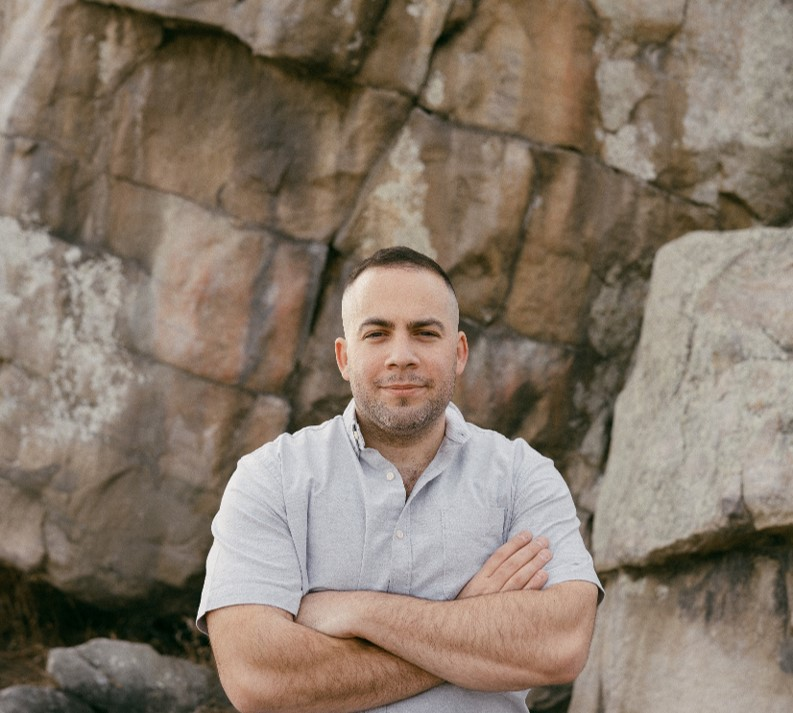
\includegraphics[width=0.65\textwidth]{images/resume_profile_picture.jpg}\hfill\null

\vspace*{0.5ex} % Extra space after the picture

\headleft{Profile Summary}
Dynamic and results-driven professional with over 8 years of experience in \textit{ technical solutions sales} specializing in Public and Private Cloud. Proven track record of exceeding quotas and building strong relationships, particularly within Federal verticals. Adept at guiding customers through the full sales cycle and dedicated to accelerating sales growth while cultivating enduring partnerships.

\headleft{Contact details}
\small % To fit more content
\MVAt\ {\small ajammes.ftnt@gmail.com} \\[0.4ex]
\faGithub\ {\small github.com/AJLab-GH}\\[0.2ex]
\Mobilefone\ +1\,613\,889\,6564\,\\

\normalsize

\headleft{Personal information}
Citizenship: \textbf{Canadian} \\[0.5ex]
Clearance: \textbf{Secret (2026), Top-Secret Elligibility} \\[0.5ex]
Languages: \textbf{English}, \textbf{French}

\headleft{Skills}
\begin{itemize}
\item Azure, Amazon Web Services, Google Cloud Platform, Oracle Cloud Infrastructure
\item Terraform, AWS CloudFormation, Azure Resource Manager (JSON, BICEP)
\item Docker, Kubernetes, AKS, EKS
\item Azure Pipelines, AWS Code Pipeline, Azure DevOps, Jenkins
\item Git, Devcontainers, CPSM, CWPP, CIEM, CNAPP
\end{itemize}

\end{minipage}%
\kern0.09\textwidth\relax%%Right margin provided explicitly to stretch the colourbox
}
\end{minipage}% Right column
\hskip2.5em% Left margin for the white area
\begin{minipage}[t]{0.61\textwidth}
\setlength{\parskip}{0.8ex}% Adds spaces between paragraphs; use \\ to add new lines without this space. Shrink this amount to fit more data vertically

\vspace{2ex}

\headright{Experience}

\textsc{\textbf{Consulting System Engineer --- Cloud Architect} \textbf{at} \textbf{Fortinet (Canada).} \dates{2022.04--Present}} \\

\small{Strategic Sales Support: Acted as a key technical resource for strategic pre-sales engagements across Canada, collaborating with Fortinet Sales teams to design and recommend tailored security solutions, ensuring optimal customer satisfaction.}

\is
\small{Customer and Partner Engagements: Led high-impact technical meetings, presentations, and product demonstrations for customers and channel partners, highlighting Fortinet's strengths.}

\is
\small{Solution Architecture and Design: Partenered with SE peers to architect secure IP networks, leveraging all facets of Fortinet's product line to deliver superior solutions in competitive scenarios.}

\is
\small{Technical Consultancy: Served as a subject-matter expert in pre-sales design reviews, providing technical guidance to internal stakeholders to drive positive customer outcomes in competitive scenarios.}

\is
\small{Training \& Mentorship: Led nationwide training for System Engineers and mentored SE specialists within Virtual Teams to enhance technical skills.}

\is
\small{Cross-functional Collaboration: Collaborated with Engineering to identify, qualify, and develop key features that strengthen Fortinet's market position.}

\is
\small{Technical Documentation: Developed comprehensive technical guides to streamline product demonstrations and emphasize Fortinet's advantages.}

\vspace{2ex}
\textsc{\textbf{Presales Security Expert --- Cloud Architect} \textbf{at} \textbf{Fortinet (Federal).} \dates{2019.06--2022.04}} \\

\small{Sales Support: Acted as the primary technical resource on sales calls, educating customers on features, specifications, functionality, and integration of networking solutions.}

\is
\small{Strategic Cloud Partnerships: Established key partnerships with cloud service providers, collaboratively selling, deploying, and delivering integrated solutions that expedited the Security Assessment & Authorization (SA\&A) process, enabling customers to quickly attain their Authority to Operate (ATO) and achieve operational readiness in the cloud.}

\is
\small{Federal Sector Selling: Successfully sold tailored solutions to the Federal vertical, enhancing company presence in the sector.}

\is
\small{High-Value Deals: Closed multiple significant deals, driving substantial revenue growth.}

\is
\small{Presentations: Delivered persuasive presentations to C-suite executives and team members, securing buy-in across all levels of the organization.}

\vspace{2ex}
\textsc{\textbf{Diamond Services Engineer \& TAC} \textbf{at} \textbf{Check Point (North-America).} \dates{2017.01--2019.06}} \\

\small{Customer Engagement: Played a key role in the design, deployment, and maintenance of cloud security solutions for Fortune 100 companies. Additionally, led training on public and private cloud solutions for both internal stakeholders and customers across Canada, the United States, and internationally.}

\headright{Education}

\textsc{Network Security Professional Program.} \textit{from Willis College}. \dates{2015--2016} \\

\headright{Fun Facts}

\textit{This resume was created and delivered as Code.}

\end{minipage}

\end{document}
